\chapter{Reporting results}
\label{ch:reportingresults}

%
% Een scriptie is een afgesloten geheel. Alle informatie die nodig is om het onderwerp ten gronde te begrijpen moet er in zitten. Het mag dus niet nodig zijn om nog externe bronnen na te lezen voordat je de tekst kan begrijpen.
% Dat betekent o.a. dat je specifieke vaktermen binnen het domein moeten verklaard worden!

At a certain point you have collected and analyzed a lot of information, and it is time to prepare the final document. In this chapter you will find some tips and guidelines to achieve a good result.

In this guide, we limit ourselves to a few key points and specific recommendations for formatting the text in {\LaTeX}. A more comprehensive overview can be found in the book by~\textcite{Pollefliet2011}.

\section{General guidelines}
\label{ch:generalguidenlines}

When you write a text, you want to put some effort in making it as pleasant as possible to read. However, there are a few things to keep in mind. In your bachelor's thesis you demonstrate that you have a professional attitude and a healthy dose of maturity. This should also be reflected in your writing style. The text must appear professional and objective. In particular, avoid the following:

\begin{itemize}
  \item Writing from your own point of view is out of the question. So never use the \textbf{I-form}. After all, it gives the impression that you are giving your \emph{own opinion}, and as a junior in your field you don't have enough authority for that. The claims you make in your bachelor's thesis must be objectively demonstrable facts, which are either supported by a reference to authoritative professional literature or follow from your own research results.
  \item Do not use \textbf{colloquial} language.  Stay formal and business like.
  \item Do not use \textbf{vague terms} to indicate a quantity, eg long, large, fast, popular, \ldots Quantify all these statements with numbers and units of measurement (supported of course by literature references or own research results).
  \item Do not use the \textbf{future tense.} The moment your finished bachelor's thesis is read, it is a report of research carried out in the past. So not ``First will be looked at\ldots'' but ``First was examined\ldots''
\end{itemize}

% http://www.taalwinkel.nl/schrijfproces/een-wetenschappelijke-schrijfstijl/
% familiair (je), ``populariserend''

% Voorbeeld vage termen:
% ``Doorheen de laatste jaren zijn mobiele applicaties enorm ge-
% groeid''
% Bron -> http://blog.appfigures.com/app-stores-growth-accelerates-in-2014/
% Gebruik waar mogelijk Nederlandse termen en vermijd Anglicanismen. Als er een Nederlands woord voor bestaat gebruik je dat, en niet de Engelse term. Bv. tree -> boom, deployen -> uitrollen, enz.

% Een zin = een gedachte
% Een paragraaf = bij elkaar horende gedachten die één onderwerp, redenering vormen
% Tip: De eerste zin van een paragraaf bevat de hoofdgedachte van de paragraaf, de andere zinnen leggen die verder uit, of gaan er dieper op in.
%
% Samengestelde woorden hangen aan elkaar: informatiebeveiliging ipv informatie beveiliging

Keep your \emph{target audience} in mind. In principle, you can assume that the reader has an ICT background (unless you are developing your subject in collaboration with or on behalf of someone from another discipline). You can therefore usually assume a certain basic knowledge, but you should certainly explain terms and abbreviations that are specific to your own research domain.

Do a \emph{thorough check} for spelling and grammatical errors. These \emph{must} be corrected when submitting. For a computer scientist, every dot and comma counts. A text full of errors gives a very bad impression about your abilities.

Start each chapter (and section) with an introductory paragraph that outlines its content and links to the previous chapter. Someone who immediately starts reading that chapter gets some context that way.


% Volgorde van schrijven (samenvatting laatste)

%- Conclusie, samenvatting, voorwoord schrijf je het laatste maar het is vaak het eerste dat gelezen wordt. Bijzonder veel aandacht aan schenken
    %- Conclusie moet terug grijpen op de onderzoeksvraag
    %- Bedenkingen, future work
    %- Samenvatting is geen voorwoord. Moet maw. ook belangrijkste conclusies bevatten

% LaTeX tips
%
% Aanhalingstekens: er bestaan geen smart quotes
% - links: backquote, rechts single quote
% - dubbele aanhalingstekens: `` en ''

% Titel:
% - concreet, niet enkel het onderzoeksdomein benoemen
% - Geef het onderwerp, niet een onderzoeksvraag
% - Gebruik geen afkortingen en vermijd jargon
% - Vermijd algemene, nietszeggende woorden. vb. ``Studie,''  ``Onderzoek naar'' -> een bachelorproef is altijd een onderzoek

% Einde inleiding: Sectie ``Opzet van deze bachelorproef''
% De rest van deze bachelorproef is als volgt opgebouwd:
%
% In hoofdstuk N \ldots
% In hoofdstuk N+1 \ldots
% \ldots

\section{Images}
\label{sec:images}

Inserting images into a {\LaTeX} document is one of the stumbling blocks for novice users of the typesetting system. In a classic WYSIWYG word processor you are used to determining where an image will end up on the paper. Usually you do that immediately below the part of the text where the image is referenced. In a larger document, this becomes problematic. After all, it is possible that by adding text before the image, it will exceed the bottom margin. The word processor may then move the image to the next page and you will get extra white space at the bottom. This will not look good, and you will lose valuable time positioning the images correctly in relation to the text.

{\LaTeX} can determine itself where an image is best positioned. It is initially annoying to have to relinquish this control, but the page mirror will look a lot better because of it. Sometimes {\LaTeX} chooses to place the image a page further or earlier than the text that relates to it. This means that the context for the image is no longer with the image. However, you can solve this by adding a caption (\emph{caption}) to each image that fully describes what can be seen in the image. Don't limit yourself to a few words. Use complete sentences so that the reader can understand the image without having to search for the accompanying text. In the text itself you then refer to the image (with \verb|\ref{fig:label}|).

% TODO: template voor invoegen van afbeelding

Under copyright law it is permitted to copy images from other publications within the context of education without the prior permission of the author. It is then of course essential that you add a literature reference in the caption. Otherwise, this is considered plagiarism.

Adding product or company logos is \emph{not} a good idea. After all, this does not only fall under copyright law, but also under the trademark law. A logo reflects the identity of a company and the use of the logo is therefore strongly controlled (size, correct use of color, etc.). Third parties may only use the logo after explicit permission and under specific conditions. In a thesis, a logo does not add any substantive added value, which in itself is a reason not to include one.

When you copy an image from a website, make sure that the resolution is high enough. Images that look good on a monitor can clearly show the individual pixels on paper, which doesn't look good. A display typically has a much lower resolution (96 DPI or \emph{dots per inch}, pixels per inch) than a printer (300 or 600 DPI). For a good result, an image must contain at least as many pixels as the desired height or width of the image on paper, multiplied by the resolution. So, for example, if you want to print an image at $5 \times 5$ cm (or about 2 inches) on a 300 DPI printer, your image must be at least $600 \times 600$ pixels in size.

An alternative is to work with \emph{vector graphics}, i.e. figures that are drawn in the document using mathematically defined shapes. There is a very extensive package for {\LaTeX} for this: Ti$k$Z. This does have a steep learning curve, but the result is of a high quality. An introduction to Ti$k$Z is beyond the scope of this guide, but there are many tutorials and examples available on the Internet\footnote{For example \url{http://www.texample.net/tikz/}}.

% Voldoende hoge resolutie voor screenshots (gekopieerd van webpagina): http://brandonmathis.com/blog/2010/10/08/how-to-get-high-resolution-screenshots-of-a-website
% Kleurenpallet (contrast, toeg
% tikz (maar dat is een specialiteit op zich\ldots)
%
% Index? Woordenlijst?

% TODO: SECTIE: de literatuurstudie schrijven
%
% De literatuurstudie/state-of-the-art is een doorlopende tekst waarin je in je eigen woorden de situatie in het onderzoeksdomein schetst, met op gepaste plaatsen verwijzingen naar de literatuur. Expliciet schrijven ``in het artikel X van Y heb ik Z gelezen'' wordt niet gedaan. Lees een aantal wetenschappelijke publicaties over je onderwerp en probeer die stijl na te volgen.
%
% Wanneer verwijzen naar de literatuur:
% - Elke introductie van domeinspecifieke vaktermen
% - Elke bewering over het vakdomein (die je quantificeert!)
% - Elke verwijzing naar resultaten vorig onderzoek
%
% Twee commando's: (Auteur, jaar) of Auteur (jaar)


\section{Numbers visualisation }
\label{sec:numbersvisualisation}

In the Data Science \& AI course, good visualization of numbers is discussed in detail and practiced. Nevertheless, we see that a lot of mistakes are still made in the bachelor's thesis, resulting in incorrect conclusions. That is why we will come back to this topic here.

% - Enkel gemiddeldes vermelden is onvoldoende! Minstens ook standaardafwijkingen geven en statistische toetsen uitvoeren om te verifiëren of resultaten significant verschillen.

Suppose you execute a performance comparison between two systems, A and B. You have performed an experiment 50 times on each system and recorded the results. Let us suppose that the result of the measurement is a

\begin{figure}
  \begin{subfigure}{.5\textwidth}
    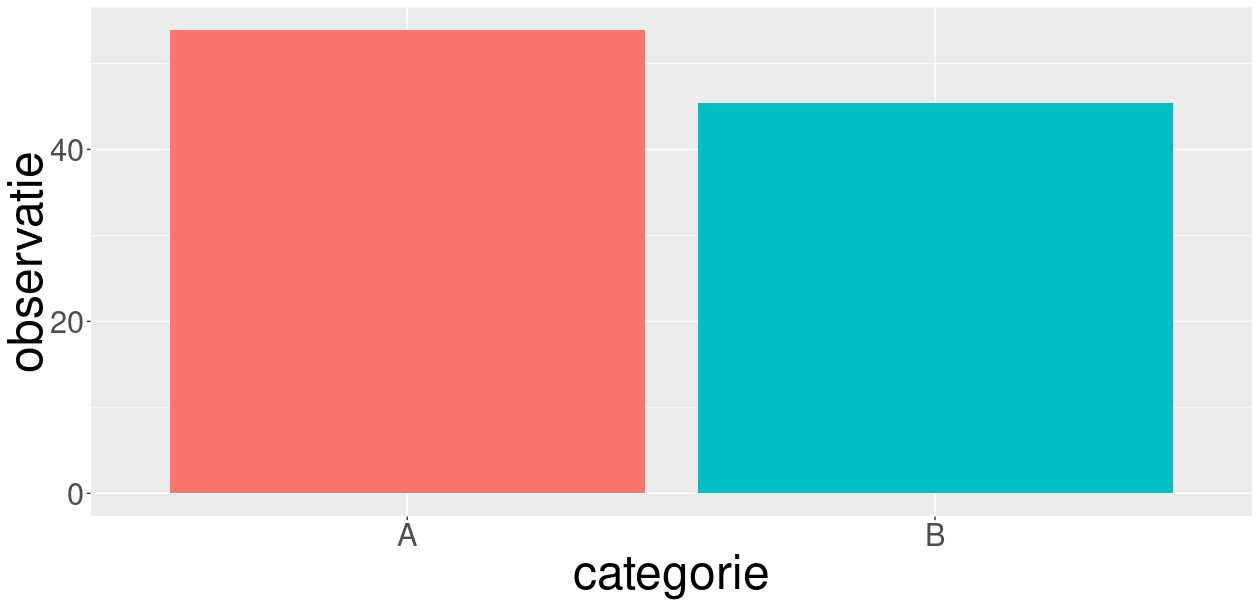
\includegraphics[width=\textwidth]{examples/barplot.png}
    \caption{Bar chart of averages. This is not enough to draw a conclusion}
    \label{fig:barplot}
  \end{subfigure}
  \begin{subfigure}{.5\textwidth}
    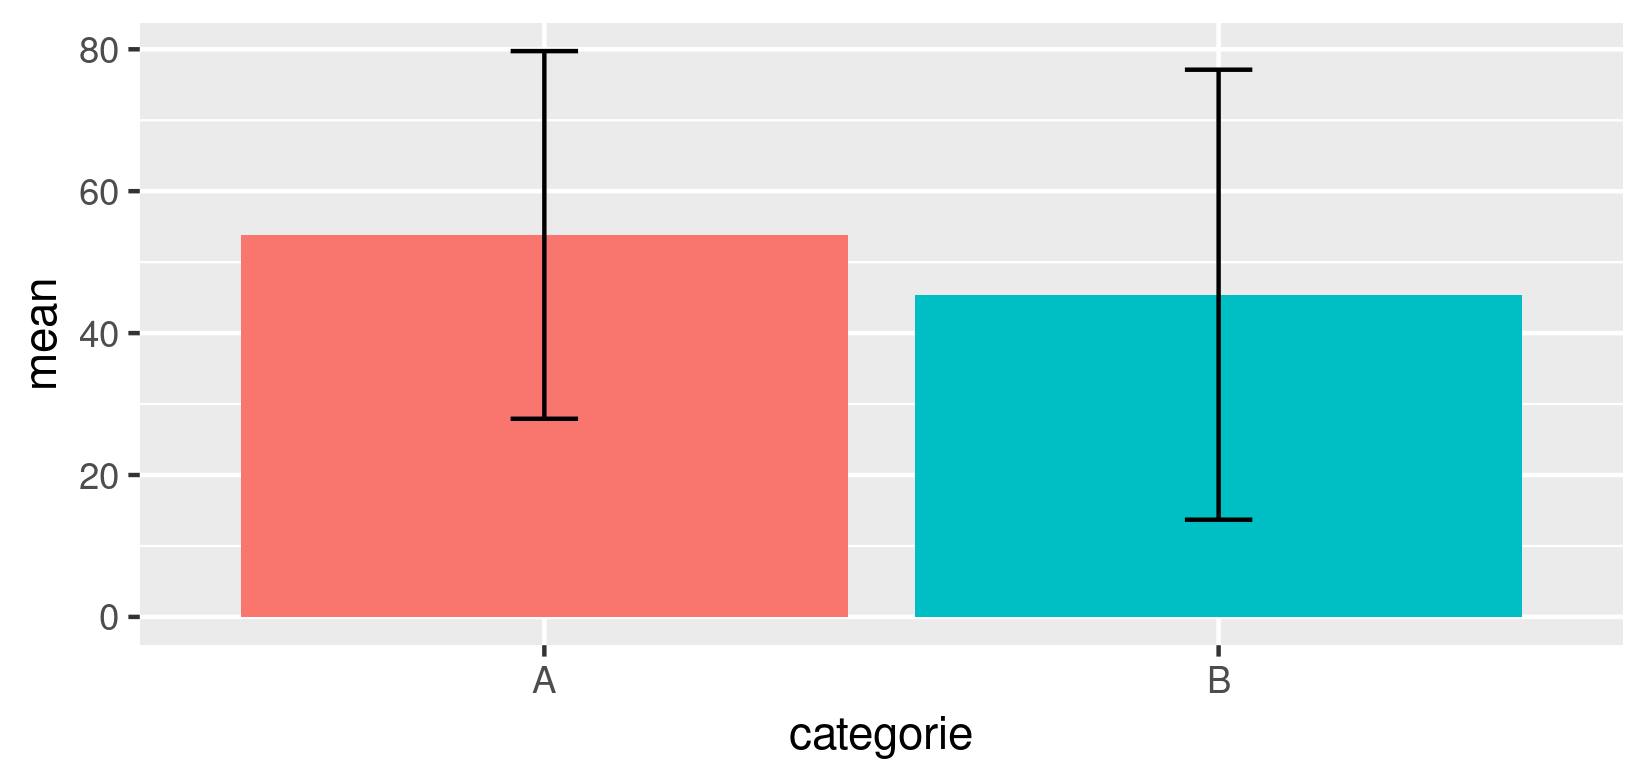
\includegraphics[width=\textwidth]{examples/barplot-errorbars.png}
    \caption{Bar chart with \textit{error bars} representing the size of the sample standard deviation. Due to the large spread, the difference between the two categories is suddenly much less pronounced.}
    \label{fig:barplot-errorbars}
  \end{subfigure}
  
  \begin{subfigure}{.5\textwidth}
    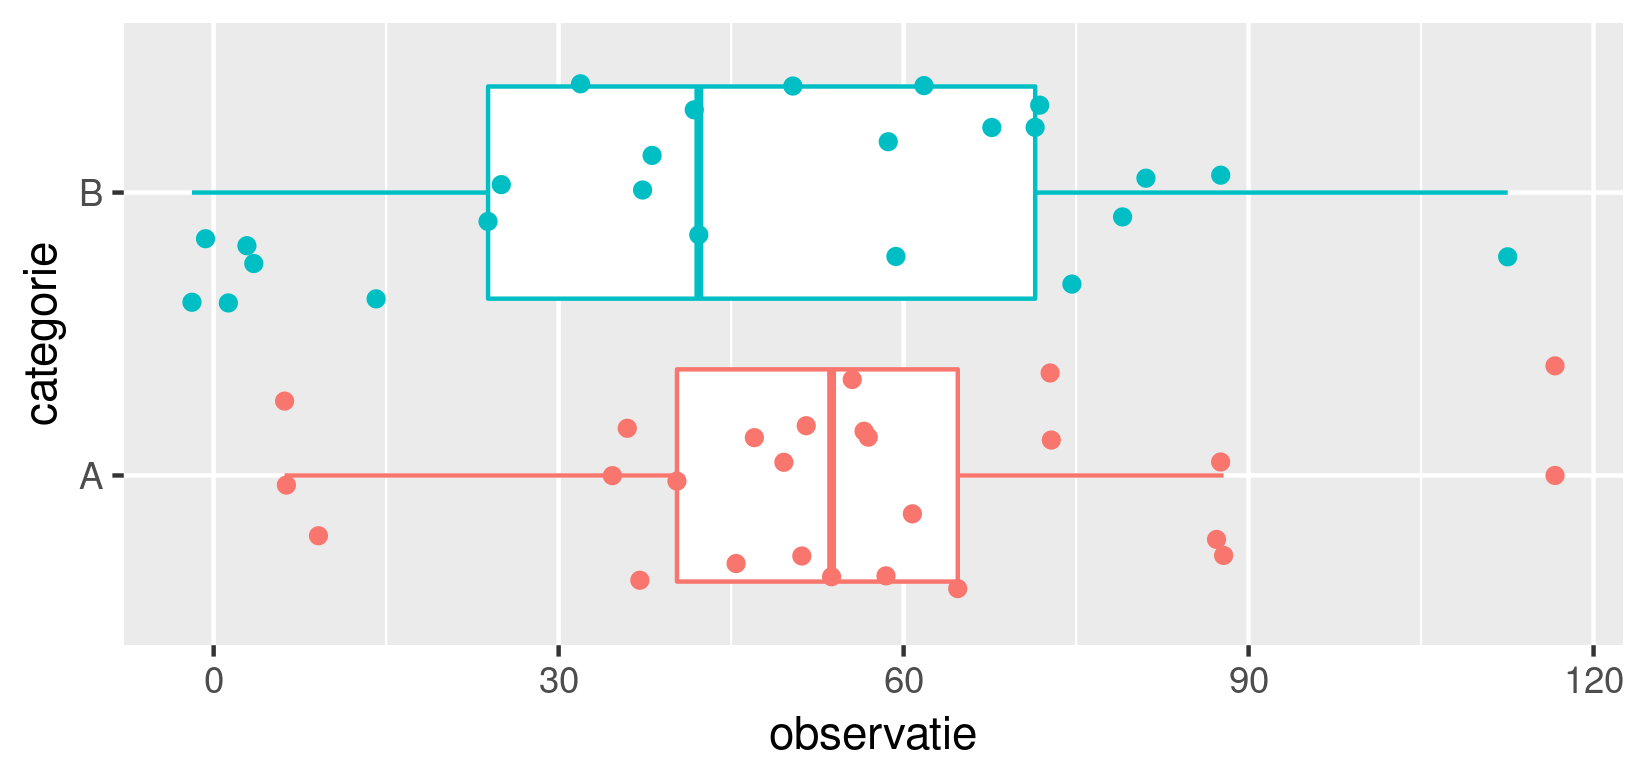
\includegraphics[width=\textwidth]{examples/boxplot-jitter.png}
    \caption{Box plot with individual observations shown as dots. This makes the spread of the data even clearer.}
    \label{fig:boxplot-jitter}
  \end{subfigure}
  \begin{subfigure}{.5\textwidth}
    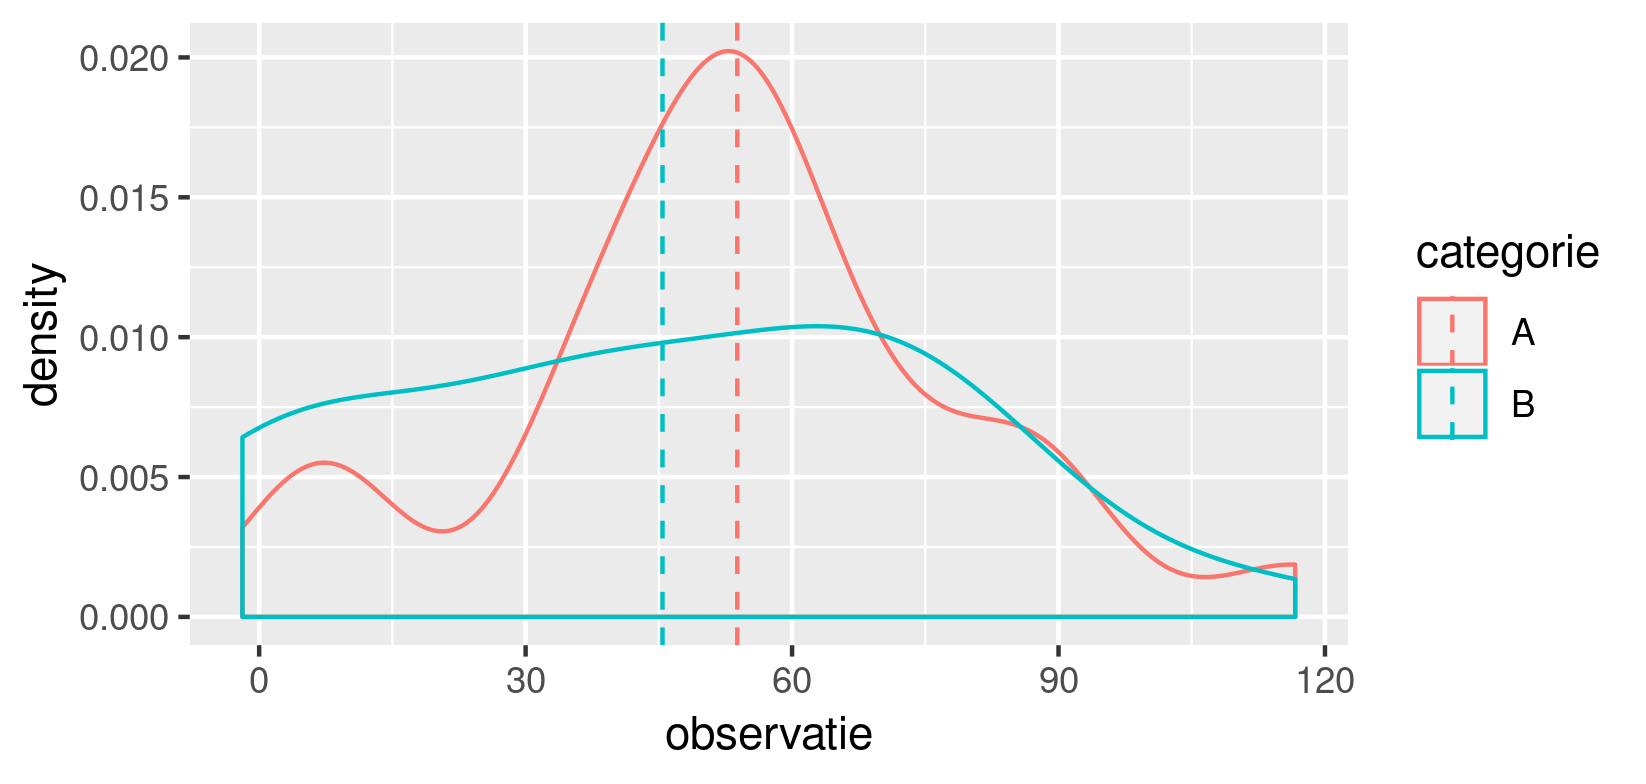
\includegraphics[width=\textwidth]{examples/density-plot.png}
    \caption{Probability density with sample means indicated as a vertical dotted line. Here it becomes clear that the results of the experiment are not normally distributed. This means that a bar chart with error bars is actually not suitable for this data.}
    \label{fig:density-plot}
  \end{subfigure}
  
 \caption[Visualize number data]{Different ways to visualize the same data.}
\end{figure}

